AS mentioned in \refSec{sec_oz_dynamic_oz}, the mobility in Dynamic \oz{} is achieved
by attaching a distinguished variable transferableOperation for location. Location transferring
is mimicked by assigning a new location to that variable. To translate the variable transferableOperation into \picalc{} we cannot use \picalc{} channel as in \refSec{sec_tra_mapping_state_variables}, since the value of transferableOperation will be a channel name and not a processes representing a value like $Zero$. Thus, we map the variable transferableOperation to channel named transferableOperation and:

\begin{itemize}
\item transferableOperation = nil is mapped to Nullref(transferableOperation).

\item transferableOperation = talk is mapped to Ref(transferableOperation,talk).
\end{itemize}
as shown in \refFig{tra_ref} \refLis{tra_ref_listing}

\begin{figure}[H]%
\centering
\subcaptionbox{transferableOperation = nil.}{\fbox{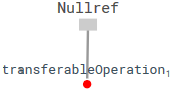
\includegraphics[keepaspectratio,width=0.45\textwidth]{./images/transformational_semantics_of_oz/transferableOperation_null.png}}}%
\hspace{\fill}
\hspace{1em}%
\subcaptionbox{transferableOperation = talk}{\fbox{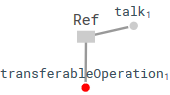
\includegraphics[keepaspectratio,width=0.45\textwidth]{./images/transformational_semantics_of_oz/transferableOperation.png}}}%
\caption{mapping transferable operation's variable}
\label{tra_ref}%
\end{figure}

\lstinputlisting[backgroundcolor=\color{white},caption={ Nullref and Ref processes in ABC code.},captionpos=b, label={tra_ref_listing}]{listings/ref_OZ.abc}